%----------------------------------------------------------------------------------------
%       CHAPTER 5
%----------------------------------------------------------------------------------------

\cleardoublepage

\chapterimage{oceanacidification.png} % Chapter heading image

\chapter{Fossil fuel CO$_{2}$ and 'ocean acidification'}\label{ch:fossil-fuel-co2}

\hfill \break

%------------------------------------------------
\newpage
%------------------------------------------------

\section*{Readme}

You will need to download a new \textit{restart} file prior to embarking on the experiments. This preindustrial spin-up includes a basic ocean (-atmosphere) carbon cycle. It follows the physical climate configuration of \textit{Cao et al.} [2009] but to simplify your introduction of carbonate chemistry, does not include biology (or associated e.g., nutrient tracer).

\vspace{2mm}

\noindent To fetch this: change to the \textsf{\footnotesize cgenie\_output} directory, and type (or copy-paste with care\footnote{\uline{ALL one line with a space before the URL.}}):
\vspace{-2mm}\small\begin{verbatim}
$ wget --no-check-certificate 
   http://www.seao2.info/cgenie_output/cookie.CB.p_worjh2.rCARB.SPIN.tar.gz
\end{verbatim}\normalsize\vspace{-2mm}

\noindent Extract the contents of this archive by typing:
\vspace{-2mm}\small\begin{verbatim}
$ tar xfzv cookie.CB.p_worjh2.rCARB.SPIN.tar.gz
\end{verbatim}\normalsize\vspace{-2mm}
\noindent (and then change directory back to \textsf{\footnotesize genie-main} to run the model)

%------------------------------------------------
\newpage
%------------------------------------------------

\section{Exploring the consequences of fossil fuel CO$_{2}$ emissions}

For the next experiment(s) you can chuck \(CO_{2}\) into the atmosphere, just for the hell of it. As much as you want! Apparently, humans are actually doing this now. Imagine that!

\vspace{1mm}

A new \textit{user-config} is provided -- \textsf{\footnotesize\ LAB.5.1.EXAMPLE} -- which unlike experimental setups in previous Chapters, is configured with climate being responsive to any changes in atmospheric \(CO_{2}\) (i.e., it takes account of \(CO_{2}\)-climate feedback). (We can make this choice because now we are going to calculate atmospheric $CO_{2}$.) The setting (near the top of the \textit{user-config} file) that does this is:
\vspace{-2pt}\small\begin{verbatim}
# set CO2-climate feedback
ea_36=y
\end{verbatim}\normalsize\vspace{-2pt}
(Previously it was disabled (\texttt{\small ea\_36=n}) and climate was fixed at a given radiative forcing equivalent, set by parameter \texttt{\small ea\_radfor\_scl\_co2}.)

\vspace{1mm}
Additional (netCDF) output has also been prescribed, via the \textit{user-config} parameter setting: \texttt{\small bg\_par\_data\_save\_level=10} so that more data relevant to assessing ocean acidification is saved.

%------------------------------------------------
\vspace{1mm}\noindent\rule{4cm}{0.1mm}\vspace{2mm}
%------------------------------------------------

\noindent First, you should start with a control experiment to provide a baseline response (or hopefully, lack of response) to which you can contrast your perturbation experiments. It is also a good experiment to interrogate and explore new output and concepts (i.e., carbonate chemistry). For this, copy and rename\footnote{e.g., \textsf{LAB.5.1.control}} the example \textit{user-config} for this section -- \textsf{\footnotesize\ LAB.5.1.EXAMPLE}.

\small\begin{verbatim}
$ ./runcookie.sh cookie.CB.p_worjh2.rCARB LABS LAB.5.1.control 10 
   cookie.CB.p_worjh2.rCARB.SPIN
\end{verbatim}\normalsize

\noindent Now, run an actual experiment. The \textit{user-config} \textsf{\footnotesize\ LAB.5.1.emissions} is almost identical to your control experiment, except it specifies a release of \(CO_{2}\) to the atmosphere, which by default is set to a value of just \(1\:PgC\) (cf. current emissions are ca. \(10\:PgC\:yr^{-1}\)) and over an interval of just a single year. (Releasing \(CO_{2}\) just over a single year is obviously rather unrealistic and many impacts will decay away rapidly, but represents a useful idealized experiment for assessing the time-scale(s) of fossil fuel \(CO_{2}\) uptake by the ocean.)

Run for e.g., 10 years (or for somewhat longer if you like but make sure that you have a \textit{control} experiment of the same length) and also starting from the preindustrial \textit{re-start} experiment \textsf{\footnotesize cookie.CB.p\_worjh2.rCARB.SPIN}, i.e.:
\small\begin{verbatim}
$ ./runcookie.sh cookie.CB.p_worjh2.rCARB LABS LAB.5.1.emissions 10 
   cookie.CB.p_worjh2.rCARB.SPIN
\end{verbatim}\normalsize

\noindent \textbf{A summary of relevant \textit{time-slices} and \textit{time-slice} output is given in the Appendix to this Chapter.}

\vspace{1mm}

\noindent What specific model results variables to consider … ? Obviously atmospheric $CO^{2}$ to start with. Think about the climate change and ocean acidification literature and which environmental (physical and geochemical) properties are considered either critical for ecosystems or are simply helpful and/or illustrative. In the 3-D netCDF \textit{time-slice} file remember, for instance, that ocean surface waters in which aragonite becomes under-saturated (OHMEGA < 1.0) is regarded as a critical threshold for organisms making aragonite shells and skeletons and spells TROUBLE for some poor calcifying marine organism somewhere. For climate change ... the variables of particular interest should be obvious. Remember that there are both \textit{time-series} outputs, as well as  2D and 3D fields, any or all of which might be  helpful for elucidating impacts.

%------------------------------------------------
\newpage
%------------------------------------------------

\subsection{Idealized emissions forcing}

\noindent The default settings in the experiment that you have just run was for $1\:PgC\:yr^{-1}$ over a single year (i.e., an idealized pulse of unit size and duration). You can easily modify the experimental design to release more/less \(CO_{2}\) very much as you did for the red dye tracer. In the \textit{user-config} file, the line:
\vspace{-2pt}\small\begin{verbatim}
bg_par_atm_force_scale_val_3=8.3333e+013
\end{verbatim}\normalsize\vspace{-2pt}
scales the time-history of the  \(CO_{2}\) flux, given in the forcing file:

\vspace{2pt}
\noindent \textsf{\footnotesize biogem\_force\_flux\_atm\_pCO2\_sig.dat}
\vspace{2pt}

\noindent ... which can be found in the directory:

\vspace{2pt}
\noindent \textsf{\footnotesize cgenie.cookie/genie-forcings/pyyyyz.FpCO2\_Fp13CO2}
\vspace{2pt}

\vspace{2pt}
\noindent The format of this file is:
\vspace{-2pt}\footnotesize\begin{verbatim}
-START-OF-DATA-
     0.0  1.0
     1.0  1.0
     1.0  0.0
999999.9  0.0
-END-OF-DATA-
\end{verbatim}\normalsize\vspace{-2pt}

\noindent and defines an emission of \(1 mol C\) (carbon) per year over the first year (year 1.0) of the model experiment (between year \texttt{0.0} and \texttt{1.0}), but which in the example \textit{user-config} is then scaled by a value of \(8.333\times10^{13}\) (by the parameter \texttt{bg\_par\_atm\_force\_scale\_val\_3}) to give a total of \(1 PgC yr^{-1}\). (Year 999999.9 has no special meaning and is simply just waaaaay into the future …)

\vspace{1mm}

Pause … and note briefly how the final \(CO_{2}\) flux is arrived at. \textbf{cookie} calculates it by multiplying the value in the forcing file (1.0) by a modifying parameter in the \textit{user-config} file (\texttt{8.3333e+13}). The total flux is hence: \(1.0 \times 8.333\times10^{13} = 8.333\times10^{13} mol CO_{2} yr^{-1}\). If you set both values as \texttt{1.0}, you’d get very little carbon released (a single mol!). If you screw up and multiply \texttt{8.3333e+013} and \texttt{8.3333e+013} together as the total flux ... you’ll soon know it as you cook the Earth … But it does not matter which parameter has value \texttt{1.0} and which scales the units (\texttt{8.3333e+013}). For now, it is simply more convenient to be able to edit the \textit{forcing} file with 'simple' numbers (and leave the large numbers and units conversion in the \textit{user-config} file).

Together, the scaling and forcing value gives a \(CO_{2}\) release of \(1 PgC yr^{-1}\) for just a single year compared to current emissions are about \(10 PgC yr^{-1}\). So, do not expect anything exciting if all you emit to the atmosphere is a single measly \(1 PgC\) (over 1 year). (The parameter: \texttt{\small bg\_par\_atm\_force\_scale\_val\_4=-27.0} specifies the carbon isotopic composition of fossil fuel carbon and can be ignored for now.)

%------------------------------------------------
\vspace{1mm} \noindent\rule{4cm}{0.1mm} \vspace{2mm}
%------------------------------------------------

\noindent If you want modify files in a forcing directory, it is good practice to copy the entire directory (in the example here: \textsf{\footnotesize pyyyyz.FpCO2\_Fp13CO2} and then copy and rename it (within the \textit{forcings} folder --\textsf{\footnotesize cgenie.cookie/genie-forcings}). And then edit the file(s) you want modified. The intention is that you always retain a copy of the original, unmodified \textit{forcing}.

Having created a forcing folder with a different name, you point to it by setting the parameter:

\vspace{-2pt}\footnotesize\begin{verbatim}
bg_par_forcing_name="MYFORCING"
\end{verbatim}\normalsize\vspace{-2pt}
where \textsf{\footnotesize MYFORCING} is whatever you called the forcing directory\\(it was originally: \texttt{\footnotesize bg\_par\_forcing\_name="pyyyyz.FpCO2\_Fp13CO2"}).

%------------------------------------------------
\vspace{1mm} \noindent\rule{4cm}{0.1mm} \vspace{2mm}
%------------------------------------------------

%------------------------------------------------
\newpage
%------------------------------------------------

\noindent The importance of the control experiment which you have already run, is that ‘accidents can happen’ and the global environmental changes induced by the massive fossil fuel \(CO_{2}\) release can obscure mistakes made in the experiment configuration (parameter values) and/or the \textit{re-start} used. The template experiment provided that you sued as a control -- \textsf{\footnotesize\ LAB.5.1.EXAMPLE} is designed to be \uline{identical} to that of the actual experiment itself (\textsf{\footnotesize LAB.5.1.emissions}) \uline{with the exception of} the scaling of the \(CO_{2}\) emissions, which is set to zero.\footnote{For completeness, the isotopic value of emitted $CO_{2}$ is also scaled to zero, but because there are no emissions in the control experiment, this does not actually achieve anything in practice.}  i.e.:
\vspace{-0pt}\small\begin{verbatim}
bg_par_atm_force_scale_val_3=0.0
\end{verbatim}\normalsize\vspace{-2pt}

\vspace{1mm}

If everything is OK with the control experiment, atmospheric \(CO_{2}\) (and climate) following on from the \textit{re-start} should be stable and there should be little (or no) drift in any of the output variables (because the \textit{spin-up} you are re-starting from should have been run to an equilibrium state and you have not changed anything in the control experiment, right?).

\vspace{1mm}

It is good practice (i.e., always do it!) to \uline{always run a control experiment} for each different type of experiment – e.g., you only need to run one control experiment for a set \(CO_{2}\) emissions experiments differing only in total carbon release of the time-history of that release. When you have run both the real and control experiment, compare the results. View (or plot) both relevant \textit{time-series} output, and create anomaly maps of key \textit{time-slice} variables in \textbf{Panoply} or \textbf{MATLAB}, using a corresponding \textit{time-slice} from the control experiment to create the experiment anomaly with.

%------------------------------------------------
\vspace{1mm} \noindent\rule{4cm}{0.1mm} \vspace{2mm}
%------------------------------------------------

\noindent OK. You might want to run something a little more exciting now. For instance, rather than
\vspace{-2pt}\footnotesize\begin{verbatim}
-START-OF-DATA-
     0.0  1.0
     1.0  1.0
     1.0  0.0
999999.9  0.0
-END-OF-DATA-
\end{verbatim}\normalsize\vspace{-2pt}
you might have:
\vspace{-2pt}\footnotesize\begin{verbatim}
-START-OF-DATA-
     0.0  1000.0
     1.0  1000.0
     1.0     0.0
999999.9     0.0
-END-OF-DATA-
\end{verbatim}\normalsize\vspace{-2pt}
for a total of \(1000 PgC\) is released over a single year. Now you should see some policy-relevant impacts occur :o)

%------------------------------------------------
\vspace{1mm} \noindent\rule{4cm}{0.1mm} \vspace{2mm}
%------------------------------------------------

\noindent You can control the shape of the emissions profile as well as its magnitude. Between the start and end ‘tags’ in the text \textit{forcing} file, the data is arranged into 2 columns: the first contains a series of tie-points for defining the timing of changes in emissions, and the 2nd column contains flux information (units of \(PgC yr^{-1}\) when scaled by the parameter parameter \texttt{bg\_par\_atm\_force\_scale\_val\_3} in the \textit{user-config}). At each time-step of the model, the \(CO_{2}\) flux to be applied to the atmosphere is interpolated between these time points.

%------------------------------------------------
\newpage
%------------------------------------------------

For instance, in the \textit{forcing} (directory) file \textsf{\footnotesize biogem\_force\_flux\_atm\_pCO2\_sig.dat}, the purpose of:
\vspace{-2pt}\footnotesize\begin{verbatim}
     0.0  1.0
     1.0  1.0
     1.0  0.0
999999.9  0.0
\end{verbatim}\normalsize\vspace{-2pt}
is to specify a uniform flux of 1.0 (scaled to \(PgC yr^{-1}\)) over the first full year of the model run, followed by a sharp turn-off to zero flux at the end of first year (and remaining zero thereafter). To extend the period of emissions – for example:
\vspace{-2pt}\footnotesize\begin{verbatim}
     0.0  1.0
    10.0  1.0
    10.0  0.0
999999.9  0.0
\end{verbatim}\normalsize\vspace{-2pt}
would result in a uniform flux lasting 10 years with a sudden cut-off and zero thereafter (i.e., once scaled by the parameter in the \textit{user-config} – \(1 PgC yr^{-1}\) over 10 years – \(10 PgC\) total emissions). 

In contrast:
\vspace{-2pt}\footnotesize\begin{verbatim}
     0.0  0.0
    10.0  1.0
    10.0  0.0
999999.9  0.0
\end{verbatim}\normalsize\vspace{-2pt}
would result in a linear ramp, starting from zero at the start of year \(0.0,\) to \(1.0 PgC yr^{-1}\) at year \(10.0\) and then suddenly ceasing and remaining at zero for the remainder of the experiment (a total \(CO_{2}\) emission of \(1\times1.0\times0.5 = 5PgC\) over 10 years).

\vspace{1mm}

To ramp up (over 10 years), and then down again (over 10 years), you would specify:
\vspace{-2pt}\footnotesize\begin{verbatim}
     0.0  0.0
    10.0  1.0
    20.0  0.0
999999.9  0.0
\end{verbatim}\normalsize\vspace{-2pt}

Try making up a few 'shapes' (and hence different experiments), maybe for the same integrated/total emissions, explore the effect of different rates of rise/fall in the release rate. And/or for the same release rate and/or duration, explore the impact of different total emissions of \(CO_{2}\). Try and think in terms of hypotheses and formulate questions to guide your experimental design/configuration. (An alternative approach is to create random scenarios and in the analysis, fish for interesting patters that could lead to knowledge and/or specific questions to be tested further, but it is better to start off with a hypothesis in mind.)

Note that you can either edit and re-use the same \textit{forcing} directory and name, modifying the file \textsf{\footnotesize biogem\_force\_flux\_atm\_pCO2\_sig.dat} each time but then losing an explicit record of how you might have set the emissions profile previously, or you can copy and rename the entire \textit{forcing} directory (and then edit \textsf{\footnotesize biogem\_force\_flux\_atm\_pCO2\_sig.dat}). If you copy and rename the entire \textit{forcing} directory, in the \textit{user-config}, you then need to specify this new forcing (directory) name, e.g.:
\vspace{-2pt}\small\begin{verbatim}
# specify forcings
bg_par_forcing_name="pyyyyz.FpCO2_Fp13CO2.NEW"
\end{verbatim}\normalsize\vspace{-2pt}
if you, for instance, called your new \textit{forcing} directory (in \textsf{\footnotesize genie-forcings }): \textsf{\footnotesize pyyyyz.FpCO2\_Fp13CO2.NEW}.\footnote{Refer to the directory map in Figure 1.1. if in doubt here.}

%------------------------------------------------
\newpage
%------------------------------------------------

\subsection{Where has my carbon gone???}

In any of the emissions experiments you have tried out, in the time-series of atmospheric \(pCO_{2}\) (file: \textsf{\footnotesize biogem\_series\_atm\_pCO2.res}) you'll undoubtedly see atmospheric \(pCO_{2}\) initially rise, but then once the emissions cease, start decaying back down again. Where is it 'going'?

Well obviously the ocean. D'uh! (At least, this is true in this particularly configuration of \textbf{cookie} without a terrestrial biosphere.) A better question would be: 'where in the ocean has it gone?', and even better: 'why there?'.

In the 3D netCDF, the variable \textsf{\footnotesize ocn\_DIC} is the total dissolved carbon inorganic concentration (\(DIC\)). Open this up ... and by slicing horizontally (e.g. start at the surface, and then slice downwards), or vertically (up through the middle of the Atlantic would be a good latitude-vertical section to create), can you 'see' where the carbon (as \(DIC\)) is going? If not ... why not? Try making the same data sections from the same year of the control experiment. \(DIC\) is everywhere in the ocean in the control, with a highly spatially variable distribution. It could be then that the carbon taken up from the atmosphere in your experiment, simply overprints too small a pattern of (fossil fuel \(DIC\)) to tell background + fossil fuel from just background. (A similar situation arose when looking for the surface temperature impact of a weakening AMOC.)

To resolve this, \uline{create difference maps} of a slice (lon-lat, or lat-depth) from your experiment at time \(t\) minus the control, also at time \(t\). Now re-evaluate whether you can tell where the fossil fuel \(CO_{2}\) is going. Why (there)? (We'll also consider this question in the next exercise.)

%------------------------------------------------
\vspace{1mm} \noindent\rule{4cm}{0.1mm} \vspace{2mm}
%------------------------------------------------

\noindent What about the other carbonate system parameters? Can you track identify patterns of uptake and ocean circulation transport. For instance \(CO_{2(aq)}\)? What about \(CO^{2-}_{3}\) (before looking, and remembering your basic carbonate chemistry, what would you expect)? (\(HCO^{2-}_{3}\) should primarily track \(DIC\).)

Are there any other carbonate system impacts you can discern? Some fields to consider might include:

\vspace{1mm}
\begin{itemize}[noitemsep]
\item \(pH\) -- variable \textsf{\footnotesize misc\_pH} 
\\(There is also a field for the hydrogen ion concentration if you really want to see it.)
\item Calcite saturation state (\(\Omega_{(cal)}\)) -- variable \textsf{\footnotesize carb\_ohm\_cal}
\item Aragonite saturation state (\(\Omega_{(arg)}\)) -- variable \textsf{\footnotesize carb\_ohm\_arg} 
\end{itemize}

%------------------------------------------------
\vspace{1mm} \noindent\rule{4cm}{0.1mm} \vspace{2mm}
%------------------------------------------------

\noindent In looking at the different fields and based on your reading of the literature (you did read the background papers, right ... ?), think about what organisms live where and what environmental (carbonate system) variables might affect them (or their prey).

%------------------------------------------------
\vspace{1mm} \noindent\rule{4cm}{0.1mm} \vspace{2mm}
%------------------------------------------------

\noindent Also see the subsection -- "\textit{Isotopic tracing of fossil fuel CO$_{2}$ uptake}".

%------------------------------------------------
\newpage
%------------------------------------------------

\subsection{Historical (real-world!) emissions forcing}

Historical and future (e.g. IPCC 'SRES') emissions scenarios can  be prescribed explicitly and simply in \textbf{cookie}. An example is given as \textit{user-config} file: \textsf{\footnotesize LAB.5.1.historical}. In this, a historical emissions forcing (technically: a prescribed concentration profile of \(pCO_{2}\) is specified by the \textit{forcing}:
\vspace{-2pt}\small\begin{verbatim}
bg_par_forcing_name=’pyyyyz.RpCO2_Rp13CO2.historical2010’
\end{verbatim}\normalsize\vspace{-2pt}
In contrast to before, no additional scaling is needed because the forcing specification directly follows the observed change in atmospheric concentration with time (in units of atm \(CO_{2}\)).

\vspace{1mm}

Note that an additional line appears in the \textit{user-config}. This is because the historical \(pCO_{2}\) transient starts in the 1700s (for which a nominal date of 1765 is often used) rather than year zero. To start \textbf{cookie} counting from year 1765 rather than year zero, a start year parameter value is specified:
\vspace{-2pt}\small\begin{verbatim}
bg_par_misc_t_start=1765.0
\end{verbatim}\normalsize\vspace{-2pt}
It is also convenient to specify a set of points in time at which data is saved that are consistent with the historical period. In the example \textit{user-config}, the addition of the parameter settings:
\vspace{-2pt}\small\begin{verbatim}
bg_par_infile_slice_name=’save_timeslice_historicalfuture.dat’
bg_par_infile_sig_name=’save_timeseries_historicalfuture.dat’
\end{verbatim}\normalsize\vspace{-2pt}
specifies a series of time points at which data is saved that aligns with historically relevant years. Try viewing the contents of these (text) files:
\vspace{2pt}
\\ \footnotesize\textsf{save\_timeslice\_historicalfuture.dat }\normalsize
\\ \footnotesize\textsf{save\_timeseries\_historicalfuture.dat }\normalsize
\vspace{2pt}
\\which can be found in the directory: \footnotesize\textsf{genie-biogem/data/input }\normalsize, to get a sense of how frequently the data will be saved, and how this differs from the default settings, which are defined in the files:
\vspace{2pt}
\\ \footnotesize\textsf{save\_timeseries.dat }\normalsize
\\ \footnotesize\textsf{save\_timeslice.dat }\normalsize
\vspace{2pt}

%------------------------------------------------
\vspace{1mm}\noindent\rule{4cm}{0.1mm}\vspace{2mm}
%------------------------------------------------

\noindent Running a transient historically-forced experiment looks like this (\uline{all one line}!):
\vspace{-2pt}\small\begin{verbatim}
$ ./runcookie.sh cookie.CB.p_worjh2.rCARB LABS LAB.5.1.historical 245
   cookie.CB.p_worjh2.rCARB.SPIN
\end{verbatim}\normalsize\vspace{-2pt}
The \texttt{245} parameter value for experiment duration (years) arises on the basis of the start year being \(1765\) (as specified by \texttt{\small bg\_par\_misc\_t\_start=1765.0}) and to give an experiment end at year \(2100\).

\vspace{1mm}

Note that from year 1765 onward, changes in atmospheric \(CO_{2}\) only rise very s l o w l y initially. Don't expect to see anything happen in 10 seconds flat because relatively few people and countries in the 1800s could be bothered to burn much more than a little local coal. You could potentially start your experiment at year 1850, changing the value of \texttt{\small bg\_par\_misc\_t\_start} and specifying shorter experiment duration (\(150\) years) if you are desperate for the End of the World to come.\footnote{Don’t forget: you could submit this experiment to the cluster and do more (idealized emissions) ‘playing’ which it runs.} 

\vspace{1mm}

\noindent Given that there is observationally-based information on the distribution of anthropogenic \(CO_{2}\) taken up by the ocean (e.g., \textit{Sabine et al.} [2004]) ... and you are running a historical transient experiment with the model driven by observed increases in atmospheric p\(CO_{2}\) ... you are in a position to critically evaluate the models ability (or lack of) to represent the future-critical process of oceanic fossil fuel \(CO_{2}\) uptake and transport by large scale ocean circulation.

\vspace{1mm}

In the 2D \textbf{netCDF} output, there is a variable for the water column integrated inventory of DIC – equivalent to the Sabine map except you will need to subtract the preindustrial background of DIC first, i.e., to create a DIC anomaly map representing only the added fossil fuel \(CO_{2}\) component of ocean DIC. The data in the Sabine paper clusters around 1994. A \textit{time-slice} centered on this year (1994.5) has been configured in the model exactly for this purpose. Your baseline state can either be from prior to \(CO_{2}\) emissions commencing at any significant rate (e.g., 1750.5) or (better), from a control experiment. Note that similar comparisons could be (and are regularly) made with other tracers such as CFCs, which provide additional insights into the patterns and time-scales of trace gas update and ocean circulation. (See: \textit{Cao et al.} [2009])

\vspace{1mm}

Observational data, re-gridded to the \textbf{cookie} grid and in netCDF format can be downloaded from: \href{http://www.seao2.org/mymuffin.html}{http://www.seao2.org/mymuffin.html} (and under the ‘got data?’ box on the left). You could for instance, compare horizontal or vertical slices (3D netCDF) and create difference (anomaly) maps. Somewhat more representative of the entire ocean is to compare (or calculate difference maps) of zonal average profiles. Unfortunately, the observations are not in the form of water column integrals and hence you cannot create difference maps of model as per the \textit{Sabine} paper … unless you use the 3D \textbf{BIOGEM} \textbf{MATLAB} plotting scripts. Examples of \textbf{MATLAB} plotting of the model \textit{vs.} observed anthropogenic anomaly are shown in Figure \ref{fig:chx-co2uptake}.

\vspace{2mm}

\begin{figure}[ht]
\begin{center}
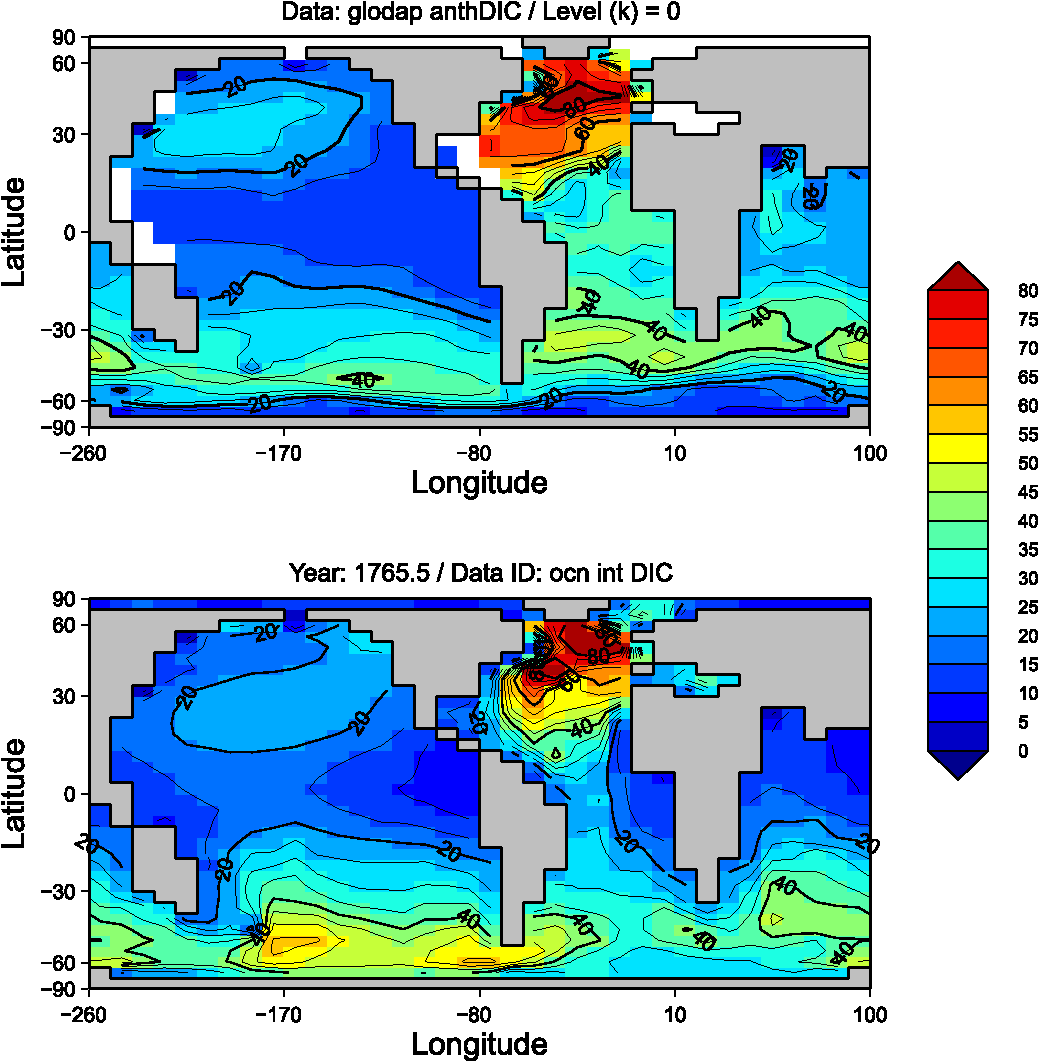
\includegraphics[scale=0.5]{chx-co2uptake.pdf}
\end{center}
\vspace{-10pt}
\caption{Observed (top) \textit{vs.} Model (bottom) anthropogenic \(CO_{2}\) inventories.
Data and model water column integrals in units of mol \(CO_{2}\) m$^{-2}$ and are nominally with respect to year 1994.}
\label{fig:chx-co2uptake}
\end{figure}

\noindent  Note that model and data are not strictly comparable in the particular configuration used here, as we do not have any biology or a 'biological pump' (more on this later) in the ocean. (The example in the figure uses the with-biology biogeochemical configuration described by \textit{Cao et al.} [2009].)

%------------------------------------------------
\newpage
%------------------------------------------------

\subsection{Assessing future carbon emissions impacts}

\noindent Finally, and the closest to being slightly interesting: rather than applying highly idealized pulses  of \(CO_{2}\) emissions, the IPCC 'SRES' emissions scenarios\footnote{Note that the past few IPCC assessment reports have switched to 'using 'RCP's -- Representative Emissions Pathways, rather than the SRES emissions scenarios -- see later Section.}  can be used to make future projections with. An example forcing of this sort is provided and can be selected by changing the name of the forcing selection parameter (\textsf{\footnotesize bg\_par\_forcing\_name}) to any one of the following:

\vspace{1mm}
\begin{itemize}[noitemsep]
\item \textsf{\footnotesize pyyyyz.FpCO2\_Fp13CO2.A1\_AIM}
\item \textsf{\footnotesize pyyyyz.FpCO2\_Fp13CO2.A1G\_MINICAM}
\item \textsf{\footnotesize pyyyyz.FpCO2\_Fp13CO2.A1T\_MESSAGE}
\item \textsf{\footnotesize pyyyyz.FpCO2\_Fp13CO2.A2\_ASF}
\item \textsf{\footnotesize pyyyyz.FpCO2\_Fp13CO2.B1\_IMAGE}
\item \textsf{\footnotesize pyyyyz.FpCO2\_Fp13CO2.B2\_MESSAGE}
\end{itemize}
\vspace{1mm}

These are 'future' emissions scenarios, which all start at year 2010, and end at year 2100. They are derived from different socio-economic and future technological assumptions in making their future emissions projections.

\vspace{1mm}

Again, as these forcings have units of \(PgCyr^{-1}\) in the time-series files, you will need to ensure that the scaling parameter in your \textit{user-config} file is set to turn units of \(PgCyr^{-1}\) into \(mol C yr^{-1}\):\footnote{For completeness also add in the specification of the isotopic composition of the carbon emissions -- refer back to the idealized experiments.}
\vspace{-2pt}\small\begin{verbatim}
bg_par_atm_force_scale_val_3=8.3333e+013
\end{verbatim}\normalsize\vspace{-2pt}

You will want to run your experiment starting from the end of the historical transient experiment you have just run rather than the original steady-state \textit{re-start}:\footnote{Note that the \textit{user-config} \textsf{\footnotesize LAB.5.1.future } is not provided for you – you will need to create this (or a file named whatever you like) by copying e.g., \textsf{\footnotesize LAB.5.1.emissions} and making the parameter changes described above (forcing specification parameter, emissions scaling parameter, and start year parameter).}
\vspace{-2pt}\small\begin{verbatim}
$ ./runcookie.sh cookie.CB.p_worjh2.rCARB LABS LAB.5.1.future 90 LAB.5.1.historical
\end{verbatim}\normalsize\vspace{-2pt}
and to run for 90 years from 20120 to 2100, set the start year to the year that the previous historical transient finished on (\(2010\)):
\vspace{-2pt}\small\begin{verbatim}
bg_par_misc_t_start=2010.0
\end{verbatim}\normalsize\vspace{-2pt}

%------------------------------------------------
\vspace{1mm} \noindent\rule{4cm}{0.1mm} \vspace{2mm}
%------------------------------------------------

\noindent You can also easily replace the details of the emissions with other SRES scenarios – simply find the year \textit{vs.} emissions rate information from the interweb\footnote{e.g., http://sres.ciesin.columbia.edu/final\_data.html} and edit or copy-and-paste the flux values for each decade into the file \footnotesize\textsf{biogem\_force\_flux\_atm\_pCO2\_sig.dat }\normalsize in the forcing directory.\textbf{ cookie} will then automatically interpolate between the decadal tie-points to give a continuous change in emissions. Now you are able to make a rather more realistic/plausible assessment of when and where potential ecological impacts (via assumed ocean chemistry criteria) might occur.

Try running (e.g. as jobs submitted to the cluster queue) some other actual or made up $CO_{2}$ emissions scenarios.

%------------------------------------------------
\newpage
%------------------------------------------------

\section{Further ideas}

Some further possibilities for investigations that build on the basic previous ones. 

%------------------------------------------------

\subsection{Assessing the importance of emissions rate}

By editing the flux magnitude and/or timing (i.e. the years that are assigned to the different forcing time-points) information of the idealized emissions \textit{forcings}, you can control the \(CO_{2}\) emissions trajectory as well as the total of fossil fuel carbon burned. Explore some different assumptions about \(CO_{2}\) release rate \uline{but for the same total carbon emitted}, and note their differing impact on climate and ocean (carbonate) geochemistry. For example rather than $1000 PgC$ over a single year (which you tested earlier), in terms of emissions rate, more realistic would be e.g., 10 or 20 \(PgCyr^{-1}\) but spread over a longer interval (order of 100 years), for the same total carbon release. For instance, one might try and address the question: “For a given total release of  fossil fuel \(CO_{2}\), is it safer to burn it slower?” The answer is maybe not completely obvious, as burning carbon resources slower will result in a small global impact, but perhaps one that persists for longer(??). You could conceive of an ensemble (related set) of model experiments, maybe one of 100 \(PgCyr^{-1}\) for 1 yr, one of 10 \(PgCyr^{-1}\) for 10 years, and one of 1 \(PgCyr^{-1}\) for 100 years, and run them all for e.g., 100 years.\footnote{These all represent rather unrealistically small total \(CO_{2}\) releases and you may want to consider a total more like 1000 \(PgC\) or rather more. You may also want to think about more realistic shapes rather than pulses, such a some sort of ramp up and then down in the emissions rate (but for the same total emissions).}

Because the experiments are getting longer to run in real time … remember to make appropriate use of the cluster queuing facility – i.e., think about whether you want to sit around starting at the screen for 15 minutes waiting for a new line of numbers appear – if not: submit to the cluster queue. (\uline{Don’t forget the control experiment}! (configured the same, except with 0 \(PgCyr^{-1}\) of emissions for 100 years).)

\vspace{1mm}

Note note that ideally you would create a new \textit{forcing} based on the original if you are editing the same original  \textit{forcing} and expecting to run different ones at the same time. Really, this is little more than you did in copying and renaming \textit{user-config} files in order to create new experiments ... except that now it involves copying and renaming entire directories in \textsf{\footnotesize genie-forcings}. Remember that the \textit{forcing} is specified by the directory name assigned to \texttt{bg\_par\_forcing\_name} (enclosed in \texttt{''}) and you will need to change this to match the name of your new \textit{forcing} directory.

%------------------------------------------------

\subsection{Determining thresholds of environmental impact}

There are various concerns about the impacts of continuing fossil fuel \(CO_{2}\) emissions and a number of proposed climatic (e.g., the \(1.5^{\circ} C \) paris protocol global warming limit often mentioned in policy documents) and ecological ‘tipping points’. You could assess the maximum allowable \(CO_{2}\) emissions to remain within particular global environmental limits in the model. For example:

\begin{itemize}[noitemsep]

\vspace{1mm}
\item What is the maximum total \(CO_{2}\) release that can be made without inducing aragonite under-saturation at the ocean surface anywhere (or any season – see Section 5.2.3 in the User Manual for seasonal time-slice data saving)? How important is the time-scale of emissions in determining this? For total emissions above this: where in the ocean does the surface first become under-saturated and what sort of (calcifying) organisms might be impacted there? How large would the emissions have to be in order to start to induce under-saturation with respect to aragonite at the surface in the tropics (home to socio-economically important reef systems)? These are questions that can be addressed with simple \(CO_{2}\) release experiments in ocean carbon cycle models and everyone seems to get a GRL paper out of it each and every time!

\vspace{1mm}
\item How important are \(CO_{2}\)-climate feedback in amplifying or diminishing future climate and ocean carbonate chemistry changes – e.g., is the same atmospheric p\(CO_{2}\) value reached with and without climate feedback (and surface warming) – if not, why? 

Hint: the solubility of \(CO_{2}\) in sea-water is a function of temperature and at higher temperatures, \(CO_{2}\) is less soluble. This means that with climate warming, \(CO_{2}\) solubility declines, less is taken up by the ocean and more is left in the atmosphere -- driving further heating in a \uline{positive feedback}.

\vspace{1mm}

All your \(CO_{2}\) emissions experiments to date have had this feedback enabled -- specified at the top of the \textit{user-config} file by:
\vspace{-2pt}\small\begin{verbatim}
# set climate feedback
ea_36=y
\end{verbatim}\normalsize\vspace{-2pt}

To quantify the role of the carbon-climate feedback, you need to run an identical emissions experiment, but with the feedback disabled:
\vspace{-2pt}\small\begin{verbatim}
# set climate feedback
ea_36=n
\end{verbatim}\normalsize\vspace{-2pt}

Note that you also to need to run a historical transient experiments with no carbon-climate feedback, if you are starting emissions experiments from the year 2010. i.e. you will have a set of future emissions experiments including the carbon-climate feedback that are run from a historical transient experiments that also includes carbon-climate feedback, vs. a set of future emissions experiments without the carbon-climate feedback that are run from a historical transient experiments that also \uline{does not include} carbon-climate feedback.

\vspace{1mm}

The importance of the feedback is simply the difference between the 2 sets of experiments, at the same year.

\vspace{1mm}
\item Also: How large a \(CO_{2}\) emission does it take to significantly ‘collapse’ the AMOC and over what time-scale? (Or alternatively: what is the atmospheric \(pCO_{2}\) threshold for AMOC collapse in \textbf{cookie}?)
\\ If the AMOC weakens or collapses … why in the absence of a prescribed freshwater perturbation does this happen? What physical process are at play in response to rapid \(CO_{2}\) release too the atmosphere that may act to reduce or shutdown deep-water formation in the ocean model? (Plotting appropriate ocean property anomalies between the \(CO_{2}\) release experiment and a control experiment might help.)
\\Related to a previous possible investigation -- does the rate of \(CO_{2}\) increase (for the same total release) matter? If so, why? What is happening in general to the structure and dynamics of the upper ocean when surface warming is very rapid?

\end{itemize}

\vspace{2mm}
\noindent Experiments could be hypothetical and consisting of \(CO_{2}\) pulses or ramps (or exponential) and run on directly from a pre-industrial spin-up, or more ‘realistic’ and run on from the end of a historical transient experiment (e.g., starting in year 2010).

%------------------------------------------------
\vspace{1mm} \noindent\rule{4cm}{0.1mm} \vspace{2mm}
%------------------------------------------------

%------------------------------------------------
\newpage
%------------------------------------------------

\noindent Also:

\begin{itemize}[noitemsep]

\vspace{1mm}
\item How much carbon can  be burned (and how quickly) such that atmospheric \(pCO_{2}\) does not increase any further and remains at some specific value (you might pick \(\times2\) or \(\times4\) preindustrial \(pCO_{2}\) (ca. 278 ppm))? This is difficult to determine well because to hold atmospheric \(pCO_{2}\)  constant, continuing emissions are required (as \(CO_{2}\) continues to be taken up by the ocean).
\vspace{1mm} 
\\One possible approach to tacking this, might be:
\vspace{1mm} 
\begin{enumerate}[noitemsep]
\item Run one or more (SRES) emissions scenarios and find the year at which your \(pCO_{2}\) threshold value is crossed. 
\item Re-run the same emissions experiment, but only for as many years as the threshold-crossing year you had identified, is reached. This will become your new \textit{re-start}.
\item Create a new experiment, with zero emissions, and run on from your new re-start. You should see atmospheric \(pCO_{2}\) start close to the value you reached at the end of the last experiment, but then decay away as the ocean continues to absorb carbon from the atmosphere. The decline in atmospheric \(pCO_{2}\) each year tells you something about the yearly emissions needed to keep atmospheric \(pCO_{2}\) constant.
\\An approximate rule-of-thump, is that \(1ppm\) in atmospheric \(pCO_{2}\) is equivalent to \(2 PgC\) (actually, a more exact conversion is \(1 ppm = 2.123 PgC\)). So you could calculate a yearly time-series of how much (in ppm) atmospheric \(pCO_{2}\) falls by each year ... convert this to PgC, and then create a new \textit{forcing}, with this as the annual emissions.
\item Create and run a new experiment, from the same \textit{re-start} experiment you created, and apply the new emissions forcing you created. See if atmospheric \(pCO_{2}\) is approximately maintained constant(?)  
\item If not sufficient constant to your satisfaction, you could also carry out a second iteration -- calculating from your latest experiment, the ppm change in \(pCO_{2}\) each year, converting to an emissions rate, and running a further experiment ...
\\Note that if you 'overhsoot' and \(pCO_{2}\) rises above the threshold value rather than falls below, you are allowed to have a \uline{negative} carbon emission to the atmosphere in your forcing.
\item The sum of the carbon emissions up to the threshold being reached, is your answer to how much more carbon can be burned and not cross that threshold ... but you will see that after that, further emissions are allowed without \(pCO_{2}\) exceeding the threshold. So the answer e.g. for year 2100 (or 2200) will be larger.
\end{enumerate}

\vspace{2mm}

There are automated ways provided in the model framework of  achieving this, and you can for instance simply tell \textbf{cookie}  to maintain a specific (or changing) value of atmospheric \(pCO_{2}\), and from this diagnose the emissions rate that was required. For instance, you'll see in the original \textit{re-start} \textit{user-config} for this chapter -- \textsf{\footnotesize cookie.CB.p\_worjh2.rCARB.SPIN} -- the \textit{forcing} used is 
\textsf{\footnotesize pyyyyz.RpCO2\_Rp13CO2}. If you go look in that forcing directory at:
\vspace{1mm}
\\\textsf{\footnotesize biogem\_force\_restore\_atm\_pCO2\_sig.dat} 
\vspace{1mm}
\\you will see a unit forcing. This is then scaled by the parameter \textsf{\footnotesize bg\_par\_atm\_force\_scale\_val\_3} to achieve a constant atmospheric \(pCO_{2}\) value of \(278 ppm\) --  \(0.278\times10^{-6} atm\). To specify a different \(pCO_{2}\) value, simple change the scaling factor (as per e.g., for the flux forcing).

The equivalent carbon emissions required to do this, are diagnosed and provided as a \textit{time-series} output (in units of \(mol C yr^{-1}\)) in file: \\\textsf{\footnotesize biogem\_series\_diag\_misc\_specified\_forcing\_pCO2.res}

\vspace{1mm}
\item Similarly -- how much more carbon can be burned but still keep global mean surface air temperature from rising beyond the 'Paris' limit of \(2^{\circ}C\) (as compared to preindustrial)?
\\This is also difficult to determine well because there are significant climate lags in the system with warming continuing even if atmospheric \(pCO_{2}\) was held constant.
\\Trial-and error would be one approach ...

\end{itemize}

%------------------------------------------------

\subsection{Future atmospheric CO$_{2}$ concentration pathways ('RCPs')}

The more recent/current incarnation of IPCC future scenarios revolves not around  making projections of future greenhouse gas emissions rates, but rather future greenhouse gas concentration pathways. (The reasoning is partly to cut out the differences in carbon cycle feedback between models, where for the same unit \(CO_{2}\) release, different climate/Earth system models might project a different atmospheric \(CO_{2}\) concentration and hence climate change (in addition to differences between models in climate sensitivity).) In \textbf{cookie}, these work pretty well much like in the historical forcing scenario, where the observed change in atmospheric \(CO_{2}\) concentration in the atmosphere with time, is prescribed and the model 'forced' to conform to this trajectory.

\vspace{1mm}

A series of RCP scenarios for how atmospheric \(CO_{2}\) concentrations may evolve with time are provided. Each actually starts at year 1765 and hence incorporates the historical transient. They can hence be used with an experiment starting at 1765 and \textit{re-starting} from a steady-state preindustrial \textit{spin-up}. Or they can be jumped into at ay point, and e.g. experiments started at year 2010, when only the year 2010 onwards part of the \(CO_{2}\) restoring \textit{forcing} is utilized. The RCP \textit{forcings} currently provided are:

\vspace{1mm}
\begin{itemize}[noitemsep]
\setlength{\itemindent}{.2in}
\item \textsf{\footnotesize pyyyyz.RpCO2\_Rp13CO2.RCP3PD}
\item \textsf{\footnotesize pyyyyz.RpCO2\_Rp13CO2.RCP4p5}
\item \textsf{\footnotesize pyyyyz.RpCO2\_Rp13CO2.RCP6p0}
\item \textsf{\footnotesize pyyyyz.RpCO2\_Rp13CO2.RCP8p5}
\end{itemize}
\vspace{2mm}
and can be selected simply by changing the name of the forcing in the \textit{user-confi}g, e.g.:
\vspace{-2pt}\small\begin{verbatim}
bg_par_forcing_name=’pyyyyz.RpCO2_Rp13CO2.RCP8p5'
\end{verbatim}\normalsize\vspace{-2pt}
\noindent which would select the RCP8.5 scenario.

\vspace{1mm}

\noindent \uline{NOTE}: ensure that
the scaling parameters are either commented out, e.g.:
\vspace{-2pt}\small\begin{verbatim}
#bg_par_atm_force_scale_val_3=8.3333e+013
#bg_par_atm_force_scale_val_4=-27.0
\end{verbatim}\normalsize\vspace{-2pt}
\noindent or simply deleted in their entirety (because the RCP forcing contains the actual values/correct units and you do not need to modify them any further).

\vspace{1mm}

The equivalent carbon emissions required to follow these concentration pathways are diagnosed by \textbf{cookie} and provided as a \textit{time-series} output (in units of \(mol C yr^{-1}\)) in file: 
\vspace{1mm}
\\\textsf{\footnotesize biogem\_series\_diag\_misc\_specified\_forcing\_pCO2.res}

%------------------------------------------------
\newpage
%------------------------------------------------

\subsection{Isotopic tracing of fossil fuel CO$_{2}$ uptake}

\noindent The  experiments on fossil fuel \(CO_{2}\) emissions to the atmosphere include an assumed isotopic composition of the emitted carbon. For any of the carbon emissions experiments you have run (including the historical transient) -- explore in the 3D output how the  isotopic composition of fossil fuel carbon is propagated from the atmosphere into the ocean and  through the ocean via its large-scale circulation. The variable you want to plot is: \textsf{\footnotesize ocn\_DIC\_13C}\footnote{Also calculated and saved are the isotopic compositions of the 3 different aqueous carbonate chemsitry components -- \textsf{\footnotesize carb\_d13C\_CO2}, \textsf{\footnotesize carb\_d13C\_CO32}, and \textsf{\footnotesize carb\_d13C\_HCO3}.}. In this, it is helpful to also take a control experiment (you did run one, right ... ?) and create a difference map to better visualize how the \(\delta^{13}C\) patterns in the ocean evolve through time.

%------------------------------------------------
\vspace{1mm} \noindent\rule{4cm}{0.1mm} \vspace{2mm}
%------------------------------------------------

\noindent By default, fossil fuel carbon is tagged with a mean fossil fuel isotopic signature of \(-27\)\permille. This in set by the parameter:
\vspace{-1mm}\small\begin{verbatim}
bg_par_atm_force_scale_val_4=-27.0
\end{verbatim}\normalsize\vspace{-1mm}
which scales the value of \(1.0\) specified in the file \textsf{\footnotesize biogem\_force\_flux\_atm\_pCO2\_13C\_sig.dat} in the \textit{forcing} directory, which in the previous fossil fuel release experiments was the \textsf{\footnotesize genie-forcing} sub-directory: \textsf{\footnotesize pyyyyz.FpCO2\_Fp13CO2}

\vspace{1mm}

To create a more pronounced 'tag' (or tracer) of fossil fuel carbon, you could, for instance, make the assumed value of the \(CO_{2}\) more negative, e.g. \(-60\)\permille would be the signature of methane (natural gas). You could also push the value even more negative and consider it an idealized numerical tracer of fossil fuel carbon (note that the lowest value you are allowed to set is \(-999\)\permille).

%------------------------------------------------
\vspace{1mm} \noindent\rule{4cm}{0.1mm} \vspace{2mm}
%------------------------------------------------

%------------------------------------------------
\newpage
%------------------------------------------------

\section{Appendix}

\subsubsection{Relevant CO2 and carbonate chemistry time-series data}

\begin{table}[ht!]
\begin{tabular}{p{0.2\linewidth} p{0.317\linewidth} p{0.4\linewidth}}
\toprule
\textbf{Filename} & \textbf{Data} & \textbf{Application}\\
\textsf{\footnotesize biogem\_series\_*.res} & &\\
\midrule

\textsf{\footnotesize atm\_p\(CO_{2}\)} & \small{Global inventory (\(mol\)), mean concentration (\(atm\)) of atmospheric \(CO_{2}\). } & \small{Drivers of and feedbacks with climate. Diagnostic of response to carbon emissions (and removal).}\\
\textsf{\footnotesize atm\_p\(CO_{2}\)\_13C} & \small{\(^{13}C\) inventory (\(mol\)) and \(\delta^{13}C\) of atmospheric \(CO_{2}\).} & \small{Diagnostic of carbon emissions (and removal). Comparison with (terrestrial) proxy \(\delta^{13}C\) data.}\\

\midrule

\textsf{\footnotesize carb\_sur\_conc\_*} & \small{Carbonate chemistry components (mean surface) (\(molkg^{-1}\)).} & \small{Not generally useful. }\\
\textsf{\footnotesize carb\_sur\_H} & \small{Surface ocean mean \([H^{+}]\) (\(molkg^{-1}\)).} & \small{More useful is pH -- reported under \textsf{\footnotesize misc} (see below). }\\
\textsf{\footnotesize carb\_sur\_ohm\_arg} & \small{Mean surface aragonite saturation.} & \small{Ocean acidification impacts of \(CO_{2}\) release. Weathering impacts. Relates to carbonate production by (modern) corals, pteropods.}\\
\textsf{\footnotesize carb\_sur\_ohm\_arg} & \small{Mean surface calcite saturation.} & \small{Ocean acidification impacts of \(CO_{2}\) release. Weathering impacts. Carbonate production by foraminifera and coccolithophorids.}\\

\midrule

\textsf{\footnotesize diag\_misc\_} \hspace{1cm} \textsf{\footnotesize specified\_forcing\_*}  & \small{Applied flux \textit{forcings} (\(molyr^{-1}\)).} & \small{Whenever a \textit{restoring}, or \textit{flux} \textit{forcing} is specified, the actual flux employed, is saved here. Useful for diagnosing the flux associated with a restoring forcing (e.g. allowing  emissions flux associated with RCP (\textit{restoring forcing}) scenario to be diagnosed.)}\\

\midrule

\textsf{\footnotesize misc\_surpH} & \small{Mean surface \(pH\).} & \small{Ocean acidification.}\\

\midrule

\textsf{\footnotesize ocn\_DIC} & \small{Global inventory (\(mol\)), mean global,  surface,  benthic concentrations (\(molkg^{-1}\)) of \(DIC\).} & \small{Carbon release and removal.}\\
\textsf{\footnotesize ocn\_DIC\_13C} & \small{Global inventory (\(mol\)), mean global,  surface, and  benthic \(\delta^{13}C\).} & \small{Carbon release and removal.}\\
\textsf{\footnotesize ocn\_ALK} & \small{Global inventory (\(mol\)), mean global,  surface,  benthic concentrations (\(molkg^{-1}\)) of \(ALK\).} & \small{'Ocean Alkalinity Enhancement' CDR.}\\

\bottomrule
\end{tabular}
\caption{Summary of the main (useful, plus notes on a few less used) \textit{time-series} output for (bio)geochemistry (non ecological) investigations.}
\end{table}

%------------------------------------------------
\vspace{1mm} \noindent\rule{4cm}{0.1mm} \vspace{2mm}
%------------------------------------------------

%------------------------------------------------
\newpage
%------------------------------------------------

\subsubsection{Relevant CO2 and carbonate chemistry time-slice data}

\begin{table}[ht!]
\begin{tabular}{p{0.15\linewidth} p{0.20\linewidth} p{0.225\linewidth} p{0.325\linewidth}}
\toprule
\textbf{variable} & \textbf{variable} & \textbf{Description} & \textbf{Application}\\
 & (long name) & &\\
\midrule

\textsf{\footnotesize carb\_ben\_ohm\_arg} \textsf{\footnotesize carb\_sur\_ohm\_cal} & \textsf{\footnotesize } & \small{Benthic aragonite and calcite saturation.} & Impacts of ocean acidification of distribution of benthic organisms. Indicator of sediment preservation.\\
\textsf{\footnotesize carb\_sur\_ohm\_arg} \textsf{\footnotesize carb\_sur\_ohm\_cal} & \textsf{\footnotesize } & \small{Ocean surface aragonite and calcite saturation.} & Impacts of ocean acidification of distribution of planktic organisms.\\

\midrule

\textsf{\footnotesize fseaair\_p\(CO_{2}\)} & \textsf{\footnotesize p\(CO_{2}\): net sea->air gas exchange flux density} & \small{Air-sea \(CO_{2}\) gas exchange.} & \small{Indicator of air-sea gas disequilibrium, regions of out-gassing/in-gassing.}\\

\midrule

\textsf{\footnotesize misc\_pH} & \textsf{\footnotesize ocean pH} & \small{Ocean surface pH.} & \small{Ocean acidification.}\\

\midrule

\textsf{\footnotesize ocn\_int\_DIC} & \textsf{\footnotesize DIC water-column integrated tracer inventory} & \small{Pattern of water column integrated ocean \(DIC\) (i.e. dissolved carbon storage) (\(molm^{-2}\)).} & \small{Indicator of \(CO_{2}\) emissions storage and transport when used in difference/anomaly maps and calculations.}\\

\bottomrule
\end{tabular}
\caption{Summary of the main (mostly useful) 2D time-slice output for (bio)geochemistry.}
\end{table}

%------------------------------------------------
\vspace{1mm} \noindent\rule{4cm}{0.1mm} \vspace{2mm}
%------------------------------------------------


%----------------------------------------------------------------------------------------
%----------------------------------------------------------------------------------------